\documentclass[10pt,aspectratio=169]{beamer}
\usetheme{metropolis}
\usepackage{booktabs}
\usepackage{graphicx}
\newcommand{\NPairs}{15}
\newcommand{\NInstances}{10}
\newcommand{\NRepos}{8}
\newcommand{\NCandidates}{22}
\newcommand{\NCaught}{7}
\newcommand{\TestCatchRate}{31.8\%}
\newcommand{\NProcessed}{20}
\newcommand{\NJudges}{2}
\newcommand{\MainFinding}{PLACEHOLDER}
\newcommand{\NPoolInstances}{1{,}216}
\newcommand{\NPoolRepos}{367}
\newcommand{\ThinkBudget}{512}
\newcommand{\MaxPromptTokens}{6{,}000}
\newcommand{\NEvalPairs}{X}
\newcommand{\NCJBPairs}{45}
\newcommand{\SpeedSmall}{X}
\newcommand{\SpeedLarge}{X}
\newcommand{\NThinkPairs}{X}

\newcommand{\RJB}{RepoJudgeBench}
\newcommand{\CJB}{CodeJudgeBench}
\newcommand{\SlideRegimeText}{Raw accuracy is at chance in both regimes: \AccRangeC{} on the single-file control, \AccRangeR{} on \RJB{}.}
\newcommand{\SlidePositionText}{Verdicts follow the slot: flip rates 71--100\%; Qwen2.5-Coder-1.5B always picks A on \RJB{}, the 4B judges almost always pick B.}
\newcommand{\SlideScalingText}{No measurable effect of diff size, files or hunks (all CIs include 0); accuracy indistinguishable from chance from \ChanceLines{} changed lines up. Authorisation regressions are missed most (\CalClsAuth{} calibrated).}
\newcommand{\SlideContextText}{Retrieved repository context: no change in raw accuracy; +\,7 to +\,22 points calibrated (significant only for Qwen3-1.7B, \CtxQwenSCal{}).}
\newcommand{\SlideThinkText}{Thinking mode (Qwen3-1.7B, 512 tokens): \ThinkQwenSCal{} points calibrated --- still not above chance.}
\newcommand{\SlideFindingTwo}{After position calibration the small judges prefer the \alert{defective} patch (\CalRCoderM{}--\CalRQwenS{}); only the 4B judges keep a weak correct signal (up to \CalRQwenM{}).}


\title{RepoJudgeBench}
\subtitle{Does LLM-as-a-Judge reliability survive the move from self-contained functions to repository-level, test-passing code changes?}
\author{Muhammad Usama \quad (25I-8007)}
\institute{Natural Language Processing --- Semester Research Project}
\date{}

\begin{document}

\maketitle

\begin{frame}{Problem definition}
\begin{itemize}
  \item LLMs are used as \alert{judges} of code: ranking agent patches, filtering training data, reward models, PR review bots.
  \item The usual oracle, the test suite, is weak at repository level: in the SWE-Bench+ audit, 32.67\% of accepted SWE-Agent+GPT-4 patches leaked the solution and 31.08\% passed only because the tests were weak (12.47\% $\rightarrow$ 3.97\% resolved after filtering).
  \item \CJB{} (base paper): 5{,}352 pairs, but every instance is \alert{single-file and test-decidable}.
\end{itemize}
\vspace{0.5em}
\textbf{Research question:} can judges still tell a correct patch from a \emph{test-passing but defective} one when the patch is a multi-file diff in a real repository?
\end{frame}

\begin{frame}{Motivation}
\begin{itemize}
  \item Defects that reviewers reject but tests do not catch: N+1 queries, races, authorisation regressions, unsafe migrations, resource leaks, swallowed errors.
  \item Judges are already load-bearing infrastructure: their errors propagate into training.
  \item Known failure modes (order sensitivity, generator sensitivity) are measured only on short, single-file code.
  \item Contamination: use pull requests created after 1 January 2025 only.
\end{itemize}
\end{frame}

\begin{frame}{Proposed solution: RepoJudgeBench pipeline}
\begin{enumerate}
  \item Real PRs ($\geq$ 2025-01-01) from SWE-bench-Live and SWE-rebench, each with a Docker image.
  \item Apply the gold patch in the container; re-render with \texttt{git diff}.
  \item \alert{AST mutation} inside the region the patch touches (6 defect classes).
  \item \alert{Admission by execution}: keep a variant only if every test that passes with the gold patch still passes.
  \item Neutral repository context from the parent commit (definitions, call sites).
  \item Pairwise judging in both orders with the \CJB{} prompt; bootstrap CIs.
\end{enumerate}
\end{frame}

\begin{frame}{Technical contributions}
\begin{itemize}
  \item A new evaluation axis: judges on \alert{repository-level, CI-passing} diffs.
  \item A CI-passing defect-injection and verification harness (\NCandidates{} candidates tested, \TestCatchRate{} caught by the PR's tests).
  \item A six-class, review-grounded defect taxonomy with executable operators.
  \item Scaling analysis (diff size, files, hunks), position bias, self-consistency.
  \item Mitigation: retrieved repository context with a budget ablation.
  \item Released: dataset, harness, prompts, raw verdict logs.
\end{itemize}
\end{frame}

\begin{frame}{RepoJudgeBench in numbers}
\begin{columns}[T]
\begin{column}{0.48\textwidth}
\begin{itemize}
  \item \NProcessed{} post-2025 tasks processed in their Docker images
  \item \alert{\NPairs{} pairs} from \NInstances{} PRs in \NRepos{} repositories
  \item median gold patch: \NGoldMedianLines{} lines, \NGoldMedianFiles{} files, \NGoldMedianHunks{} hunks
  \item \NPairsJudged{} pairs judged (no leakage, prompt $\leq$ 6k tokens)
\end{itemize}
\end{column}
\begin{column}{0.5\textwidth}
\textbf{Tests catch only \TestCatchRate{} of injected defects}
\begin{itemize}
  \item authorisation guards: \CatchAuth{}
  \item error handling: \CatchSES{}
  \item races: \CatchRace{}
  \item resource leaks: \CatchRL{}
\end{itemize}
\end{column}
\end{columns}
\end{frame}

\begin{frame}{Judging protocol}
\begin{itemize}
  \item \CJB{} pairwise prompt, verdict \texttt{[[A>B]]} / \texttt{[[B>A]]}; issue as user prompt, two unified diffs as answers.
  \item Judges: \NJudges{} open models (1.5--4B, \texttt{llama.cpp}, CPU) + a thinking condition.
  \item Forced verdict prefix $\rightarrow$ logits of \texttt{A} vs \texttt{B}: greedy verdict and $p_A$.
  \item Both orders for every pair; 95\% bootstrap CIs (resampling PRs).
  \item Control: 45 \CJB{} pairs (code generation, repair, test generation).
\end{itemize}
\end{frame}

\begin{frame}{Result 1: accuracy in the two regimes}
\centering
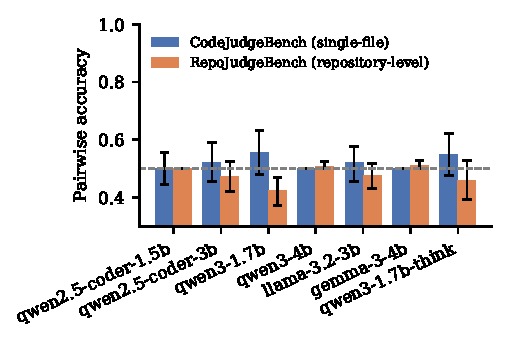
\includegraphics[width=0.62\textwidth]{../results/figures/regimes.pdf}

\small\SlideRegimeText{}
\end{frame}

\begin{frame}{Result 2: position bias and length bias}
\begin{itemize}
  \item \SlidePositionText{}
  \item After balanced position calibration, judges prefer the \alert{longer} patch in \PrefersLonger{} of unequal-length pairs.
  \item The defective variant is longer in \VarLongerShare{} of judged pairs, so judges systematically pick the defect.
  \item Benchmark artefact: a trivial ``pick the shorter patch'' rule scores \LengthHeurAcc{} --- future versions must length-match variants.
\end{itemize}
\end{frame}

\begin{frame}{Result 3: diff size and defect class}
\begin{columns}[T]
\begin{column}{0.5\textwidth}
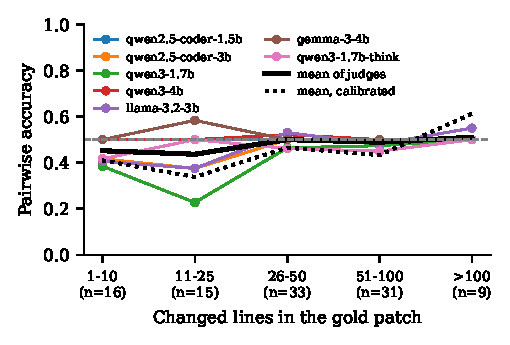
\includegraphics[width=\textwidth]{../results/figures/scaling.pdf}
\end{column}
\begin{column}{0.5\textwidth}
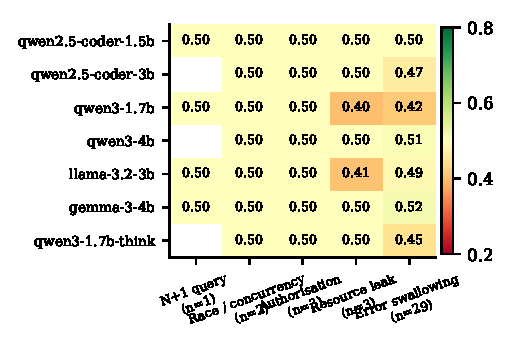
\includegraphics[width=\textwidth]{../results/figures/classes.pdf}
\end{column}
\end{columns}
\small\SlideScalingText{}
\end{frame}

\begin{frame}{Result 4: baselines and mitigation}
\begin{itemize}
  \item Static analysis with defect-targeted rules (Ruff/Bandit): \alert{\StaticRelAcc{}} --- flags the variant in \StaticRelFlagVar{} of pairs and never the gold patch.
  \item Static analysis with all rules: \StaticAllAcc{} (no signal).
  \item \SlideContextText{}
  \item \SlideThinkText{}
\end{itemize}
\end{frame}

\begin{frame}{Key findings}
\begin{enumerate}
  \item Tests miss most review-relevant defects: \TestCatchRate{} caught overall, resource leaks rarely.
  \item \SlideFindingTwo{}
  \item Verdicts are driven by \alert{position} and \alert{length}, not by the defect.
  \item Cheap targeted static analysis beats every small LLM judge on this task.
  \item Our benchmark itself has a length artefact --- a lesson for building judge benchmarks.
\end{enumerate}
\end{frame}


\begin{frame}{Limitations and deviations from the proposal}
\begin{itemize}
  \item \NPairs{} pairs from \NRepos{} repositories (proposal: $\geq$300 / $\geq$15): every task needs a multi-GB image and a test run.
  \item Only small open judges (1.5--4B) on CPU; no closed models (no API access).
  \item PR test files instead of full suites; no per-instance witness tests; no human validation yet (sheet released).
  \item N+1, migration and authorisation sites are rare in issue-resolution PRs.
\end{itemize}
\end{frame}

\begin{frame}[fragile]{Demonstration}
\begin{verbatim}
python scripts/demo.py --model models/qwen2.5-coder-1.5b-instruct-q8_0.gguf
\end{verbatim}
\begin{itemize}
  \item prints one pair: issue, injected defect, the lines where the variant differs,
  \item number of tests both patches pass,
  \item judge verdict probabilities in both orders.
\end{itemize}
All code, data and logs: \texttt{github.com/the-mgi/nlp-project-}
\end{frame}

\end{document}
